\documentclass{ximera}

\graphicspath{
  {./}
  {1-1QuantitativeReasoning/}
  {1-2RelationsAndGraphs/}
  {1-3ChangingInTandem/}
  {2-1LinearEquations/}
  {2-2LinearModeling/}
  {2-3ExponentialModeling/}
  {3-1WhatIsAFunction/}
  {3-2FunctionProperties/}
  {3-3AverageRatesOfChange/}
  {4-1BuildingNewFunctions/}
  {4-2Polynomials/}
  {5-1RationalFunctions/}
   {5-2ExponentialFunctions/}
  {6-1Domain/}
  {6-2Range/}
  {6-3CompositionOfFunctions/}
  {6-4FunctionTransformations/}
  {7-1ZerosOfFunctions/}
  {7-XZerosOfPolynomials/}
  {7-2ZerosOfFamousFunctions/}
  {8-1SystemsOfEquations/}
  {6-5FunctionTransformationsProject/}
  {1-1QuantitativeReasoning/exercises/}
  {1-2RelationsAndGraphs/exercises/}
  {../1-3ChangingInTandem/exercises/}
  {../2-1LinearEquations/exercises/}
  {../2-2LinearModeling/exercises/}
  {../2-3ExponentialModeling/exercises/}
  {../3-1WhatIsAFunction/exercises/}
  {../3-2FunctionProperties/exercises/}
  {../3-3AverageRatesOfChange/exercises/}
  {../5-2ExponentialFunctions/exercises/}
  {../4-1BuildingNewFunctions/exercises/}
  {../4-2Polynomials/exercises/}
  {../5-1RationalFunctions/exercises/}
  {../6-1Domain/exercises/}
  {../6-2Range/exercises/}
  {../6-3CompositionOfFunctions/exercises/}
  {../7-1ZerosOfFunctions/exercises/}
  {../7-XZerosOfPolynomials/exercises/}
  {../7-2ZerosOfFamousFunctions/exercises/}
  {../6-4FunctionTransformations/exercises/}
  {../8-1SystemsOfEquations/exercises/}
  {../6-3FunctionTransformationsProject/exercises/}
}

\DeclareGraphicsExtensions{.pdf,.png,.jpg,.eps}

\newcommand{\mooculus}{\textsf{\textbf{MOOC}\textnormal{\textsf{ULUS}}}}

\usepackage[makeroom]{cancel} %% for strike outs

\ifxake
\else
\usepackage[most]{tcolorbox}
\fi


%\typeout{************************************************}
%\typeout{New Environments}
%\typeout{************************************************}

%% to fix for web can be removed when deployed offically with ximera2
\let\image\relax\let\endimage\relax
\NewEnviron{image}{% 
  \begin{center}\BODY\end{center}% center
}



\NewEnviron{folder}{
      \addcontentsline{toc}{section}{\textbf{\BODY}}
}

\ifxake
\let\summary\relax
\let\endsummary\relax
\newtheorem*{summary}{Summary}
\newtheorem*{callout}{Callout}
\newtheorem*{overview}{Overview}
\newtheorem*{objectives}{Objectives}
\newtheorem*{motivatingQuestions}{Motivating Questions}
\newtheorem*{MM}{Metacognitive Moment}
      
%% NEEDED FOR XIMERA 2
%\ximerizedEnvironment{summary}
%\ximerizedEnvironment{callout}
%\ximerizedEnvironment{overview} 
%\ximerizedEnvironment{objectives}
%\ximerizedEnvironment{motivatingQuestions}
%\ximerizedEnvironment{MM}
\else
%% CALLOUT
\NewEnviron{callout}{
  \begin{tcolorbox}[colback=blue!5, breakable,pad at break*=1mm]
      \BODY
  \end{tcolorbox}
}
%% MOTIVATING QUESTIONS
\NewEnviron{motivatingQuestions}{
  \begin{tcolorbox}[ breakable,pad at break*=1mm]
    \textbf{\Large Motivating Questions}\hfill
    %\begin{itemize}[label=\textbullet]
      \BODY
    %\end{itemize}
  \end{tcolorbox}
}
%% OBJECTIVES
\NewEnviron{objectives}{  
    \vspace{.5in}
      %\begin{tcolorbox}[colback=orange!5, breakable,pad at break*=1mm]
    \textbf{\Large Learning Objectives}
    \begin{itemize}[label=\textbullet]
      \BODY
    \end{itemize}
    %\end{tcolorbox}
}
%% DEFINITION
\let\definition\relax
\let\enddefinition\relax
\NewEnviron{definition}{
  \begin{tcolorbox}[ breakable,pad at break*=1mm]
    \noindent\textbf{Definition}~
      \BODY
  \end{tcolorbox}
}
%% OVERVIEW
\let\overview\relax
\let\overview\relax
\NewEnviron{overview}{
  \begin{tcolorbox}[ breakable,pad at break*=1mm]
    \textbf{\Large Overview}
    %\begin{itemize}[label=\textbullet] %% breaks Xake
      \BODY
    %\end{itemize}
  \end{tcolorbox}
}
%% SUMMARY
\let\summary\relax
\let\endsummary\relax
\NewEnviron{summary}{
  \begin{tcolorbox}[ breakable,pad at break*=1mm]
    \textbf{\Large Summary}
    %\begin{itemize}[label=\textbullet] %% breaks Xake
      \BODY
    %\end{itemize}
  \end{tcolorbox}
}
%% REMARK
\let\remark\relax
\let\endremark\relax
\NewEnviron{remark}{
  \begin{tcolorbox}[colback=green!5, breakable,pad at break*=1mm]
    \noindent\textbf{Remark}~
      \BODY
  \end{tcolorbox}
}
%% EXPLANATION
\let\explanation\relax
\let\endexplanation\relax
\NewEnviron{explanation}{
    \normalfont
    \noindent\textbf{Explanation}~
      \BODY
}
%% EXPLORATION
\let\exploration\relax
\let\endexploration\relax
\NewEnviron{exploration}{
  \begin{tcolorbox}[colback=yellow!10, breakable,pad at break*=1mm]
    \noindent\textbf{Exploration}~
      \BODY
  \end{tcolorbox}
}
%% METACOGNITIVE MOMENTS
\let\MM\relax
\let\endMM\relax
\NewEnviron{MM}{
  \begin{tcolorbox}[colback=pink!15, breakable,pad at break*=1mm]
    \noindent\textbf{Metacognitive Moment}~
      \BODY
  \end{tcolorbox}
}


\fi





%Notes on what envirnoment to use:  Example with Explanation in text; if they are supposed to answer- Problem; no answer - Exploration


%\typeout{************************************************}
%% Header and footers
%\typeout{************************************************}

\newcommand{\licenseAcknowledgement}{Licensed under Creative Commons 4.0}
\newcommand{\licenseAPC}{\renewcommand{\licenseAcknowledgement}{\textbf{Acknowledgements:} Active Prelude to Calculus (https://activecalculus.org/prelude) }}
\newcommand{\licenseSZ}{\renewcommand{\licenseAcknowledgement}{\textbf{Acknowledgements:} Stitz Zeager Open Source Mathematics (https://www.stitz-zeager.com/) }}
\newcommand{\licenseAPCSZ}{\renewcommand{\licenseAcknowledgement}{\textbf{Acknowledgements:} Active Prelude to Calculus (https://activecalculus.org/prelude) and Stitz Zeager Open Source Mathematics (https://www.stitz-zeager.com/) }}
\newcommand{\licenseORCCA}{\renewcommand{\licenseAcknowledgement}{\textbf{Acknowledgements:}Original source material, products with readable and accessible
math content, and other information freely available at pcc.edu/orcca.}}
\newcommand{\licenseY}{\renewcommand{\licenseAcknowledgement}{\textbf{Acknowledgements:} Yoshiwara Books (https://yoshiwarabooks.org/)}}
\newcommand{\licenseOS}{\renewcommand{\licenseAcknowledgement}{\textbf{Acknowledgements:} OpenStax College Algebra (https://openstax.org/details/books/college-algebra)}}
\newcommand{\licenseAPCSZCSCC}{\renewcommand{\licenseAcknowledgement}{\textbf{Acknowledgements:} Active Prelude to Calculus (https://activecalculus.org/prelude), Stitz Zeager Open Source Mathematics (https://www.stitz-zeager.com/), CSCC PreCalculus and Calculus texts (https://ximera.osu.edu/csccmathematics)}}

\ifxake\else %% do nothing on the website
\usepackage{fancyhdr}
\pagestyle{fancy}
\fancyhf{}
\fancyhead[R]{\sectionmark}
\fancyfoot[L]{\thepage}
\fancyfoot[C]{\licenseAcknowledgement}
\renewcommand{\headrulewidth}{0pt}
\renewcommand{\footrulewidth}{0pt}
\fi

%%%%%%%%%%%%%%%%



%\typeout{************************************************}
%\typeout{Table of Contents}
%\typeout{************************************************}


%% Edit this to change the font style
\newcommand{\sectionHeadStyle}{\sffamily\bfseries}


\makeatletter

%% part uses arabic numerals
\renewcommand*\thepart{\arabic{part}}


\ifxake\else
\renewcommand\chapterstyle{%
  \def\maketitle{%
    \addtocounter{titlenumber}{1}%
    \pagestyle{fancy}
    \phantomsection
    \addcontentsline{toc}{section}{\textbf{\thepart.\thetitlenumber\hspace{1em}\@title}}%
                    {\flushleft\small\sectionHeadStyle\@pretitle\par\vspace{-1.5em}}%
                    {\flushleft\LARGE\sectionHeadStyle\thepart.\thetitlenumber\hspace{1em}\@title \par }%
                    {\setcounter{problem}{0}\setcounter{sectiontitlenumber}{0}}%
                    \par}}





\renewcommand\sectionstyle{%
  \def\maketitle{%
    \addtocounter{sectiontitlenumber}{1}
    \pagestyle{fancy}
    \phantomsection
    \addcontentsline{toc}{subsection}{\thepart.\thetitlenumber.\thesectiontitlenumber\hspace{1em}\@title}%
    {\flushleft\small\sectionHeadStyle\@pretitle\par\vspace{-1.5em}}%
    {\flushleft\Large\sectionHeadStyle\thepart.\thetitlenumber.\thesectiontitlenumber\hspace{1em}\@title \par}%
    %{\setcounter{subsectiontitlenumber}{0}}%
    \par}}



\renewcommand\section{\@startsection{paragraph}{10}{\z@}%
                                     {-3.25ex\@plus -1ex \@minus -.2ex}%
                                     {1.5ex \@plus .2ex}%
                                     {\normalfont\large\sectionHeadStyle}}
\renewcommand\subsection{\@startsection{subparagraph}{10}{\z@}%
                                    {3.25ex \@plus1ex \@minus.2ex}%
                                    {-1em}%
                                    {\normalfont\normalsize\sectionHeadStyle}}

\fi

%% redefine Part
\renewcommand\part{%
   {\setcounter{titlenumber}{0}}
  \if@openright
    \cleardoublepage
  \else
    \clearpage
  \fi
  \thispagestyle{plain}%
  \if@twocolumn
    \onecolumn
    \@tempswatrue
  \else
    \@tempswafalse
  \fi
  \null\vfil
  \secdef\@part\@spart}

\def\@part[#1]#2{%
    \ifnum \c@secnumdepth >-2\relax
      \refstepcounter{part}%
      \addcontentsline{toc}{part}{\thepart\hspace{1em}#1}%
    \else
      \addcontentsline{toc}{part}{#1}%
    \fi
    \markboth{}{}%
    {\centering
     \interlinepenalty \@M
     \normalfont
     \ifnum \c@secnumdepth >-2\relax
       \huge\sffamily\bfseries \partname\nobreakspace\thepart
       \par
       \vskip 20\p@
     \fi
     \Huge \bfseries #2\par}%
    \@endpart}
\def\@spart#1{%
    {\centering
     \interlinepenalty \@M
     \normalfont
     \Huge \bfseries #1\par}%
    \@endpart}
\def\@endpart{\vfil\newpage
              \if@twoside
               \if@openright
                \null
                \thispagestyle{empty}%
                \newpage
               \fi
              \fi
              \if@tempswa
                \twocolumn
                \fi}



\makeatother





%\typeout{************************************************}
%\typeout{Stuff from Ximera}
%\typeout{************************************************}



\usepackage{array}  %% This is for typesetting long division
\setlength{\extrarowheight}{+.1cm}
\newdimen\digitwidth
\settowidth\digitwidth{9}
\def\divrule#1#2{
\noalign{\moveright#1\digitwidth
\vbox{\hrule width#2\digitwidth}}}





\newcommand{\RR}{\mathbb R}
\newcommand{\R}{\mathbb R}
\newcommand{\N}{\mathbb N}
\newcommand{\Z}{\mathbb Z}

\newcommand{\sagemath}{\textsf{SageMath}}


\def\d{\,d}
%\renewcommand{\d}{\mathop{}\!d}
\newcommand{\dd}[2][]{\frac{\d #1}{\d #2}}
\newcommand{\pp}[2][]{\frac{\partial #1}{\partial #2}}
\renewcommand{\l}{\ell}
\newcommand{\ddx}{\frac{d}{\d x}}



%\newcommand{\unit}{\,\mathrm}
\newcommand{\unit}{\mathop{}\!\mathrm}
\newcommand{\eval}[1]{\bigg[ #1 \bigg]}
\newcommand{\seq}[1]{\left( #1 \right)}
\renewcommand{\epsilon}{\varepsilon}
\renewcommand{\phi}{\varphi}


\renewcommand{\iff}{\Leftrightarrow}

\DeclareMathOperator{\arccot}{arccot}
\DeclareMathOperator{\arcsec}{arcsec}
\DeclareMathOperator{\arccsc}{arccsc}
\DeclareMathOperator{\sign}{sign}


%\DeclareMathOperator{\divergence}{divergence}
%\DeclareMathOperator{\curl}[1]{\grad\cross #1}
\newcommand{\lto}{\mathop{\longrightarrow\,}\limits}

\renewcommand{\bar}{\overline}

\colorlet{textColor}{black}
\colorlet{background}{white}
\colorlet{penColor}{blue!50!black} % Color of a curve in a plot
\colorlet{penColor2}{red!50!black}% Color of a curve in a plot
\colorlet{penColor3}{red!50!blue} % Color of a curve in a plot
\colorlet{penColor4}{green!50!black} % Color of a curve in a plot
\colorlet{penColor5}{orange!80!black} % Color of a curve in a plot
\colorlet{penColor6}{yellow!70!black} % Color of a curve in a plot
\colorlet{fill1}{penColor!20} % Color of fill in a plot
\colorlet{fill2}{penColor2!20} % Color of fill in a plot
\colorlet{fillp}{fill1} % Color of positive area
\colorlet{filln}{penColor2!20} % Color of negative area
\colorlet{fill3}{penColor3!20} % Fill
\colorlet{fill4}{penColor4!20} % Fill
\colorlet{fill5}{penColor5!20} % Fill
\colorlet{gridColor}{gray!50} % Color of grid in a plot

\newcommand{\surfaceColor}{violet}
\newcommand{\surfaceColorTwo}{redyellow}
\newcommand{\sliceColor}{greenyellow}




\pgfmathdeclarefunction{gauss}{2}{% gives gaussian
  \pgfmathparse{1/(#2*sqrt(2*pi))*exp(-((x-#1)^2)/(2*#2^2))}%
}





%\typeout{************************************************}
%\typeout{ORCCA Preamble.Tex}
%\typeout{************************************************}


%% \usepackage{geometry}
%% \geometry{letterpaper,total={408pt,9.0in}}
%% Custom Page Layout Adjustments (use latex.geometry)
%% \usepackage{amsmath,amssymb}
%% \usepackage{pgfplots}
\usepackage{pifont}                                         %needed for symbols, s.a. airplane symbol
\usetikzlibrary{positioning,fit,backgrounds}                %needed for nested diagrams
\usetikzlibrary{calc,trees,positioning,arrows,fit,shapes}   %needed for set diagrams
\usetikzlibrary{decorations.text}                           %needed for text following a curve
\usetikzlibrary{arrows,arrows.meta}                         %needed for open/closed intervals
\usetikzlibrary{positioning,3d,shapes.geometric}            %needed for 3d number sets tower

%% NEEDED FOR XIMERA 1
%\usetkzobj{all}       %NO LONGER VALID
%%%%%%%%%%%%%%

\usepackage{tikz-3dplot}
\usepackage{tkz-euclide}                     %needed for triangle diagrams
\usepgfplotslibrary{fillbetween}                            %shade regions of a plot
\usetikzlibrary{shadows}                                    %function diagrams
\usetikzlibrary{positioning}                                %function diagrams
\usetikzlibrary{shapes}                                     %function diagrams
%%% global colors from https://www.pcc.edu/web-services/style-guide/basics/color/ %%%
\definecolor{ruby}{HTML}{9E0C0F}
\definecolor{turquoise}{HTML}{008099}
\definecolor{emerald}{HTML}{1c8464}
\definecolor{amber}{HTML}{c7502a}
\definecolor{amethyst}{HTML}{70485b}
\definecolor{sapphire}{HTML}{263c53}
\colorlet{firstcolor}{sapphire}
\colorlet{secondcolor}{turquoise}
\colorlet{thirdcolor}{emerald}
\colorlet{fourthcolor}{amber}
\colorlet{fifthcolor}{amethyst}
\colorlet{sixthcolor}{ruby}
\colorlet{highlightcolor}{green!50!black}
\colorlet{graphbackground}{white}
\colorlet{wood}{brown!60!white}
%%% curve, dot, and graph custom styles %%%
\pgfplotsset{firstcurve/.style      = {color=firstcolor,  mark=none, line width=1pt, {Kite}-{Kite}, solid}}
\pgfplotsset{secondcurve/.style     = {color=secondcolor, mark=none, line width=1pt, {Kite}-{Kite}, solid}}
\pgfplotsset{thirdcurve/.style      = {color=thirdcolor,  mark=none, line width=1pt, {Kite}-{Kite}, solid}}
\pgfplotsset{fourthcurve/.style     = {color=fourthcolor, mark=none, line width=1pt, {Kite}-{Kite}, solid}}
\pgfplotsset{fifthcurve/.style      = {color=fifthcolor,  mark=none, line width=1pt, {Kite}-{Kite}, solid}}
\pgfplotsset{highlightcurve/.style  = {color=highlightcolor,  mark=none, line width=5pt, -, opacity=0.3}}   % thick, opaque curve for highlighting
\pgfplotsset{asymptote/.style       = {color=gray, mark=none, line width=1pt, <->, dashed}}
\pgfplotsset{symmetryaxis/.style    = {color=gray, mark=none, line width=1pt, <->, dashed}}
\pgfplotsset{guideline/.style       = {color=gray, mark=none, line width=1pt, -}}
\tikzset{guideline/.style           = {color=gray, mark=none, line width=1pt, -}}
\pgfplotsset{altitude/.style        = {dashed, color=gray, thick, mark=none, -}}
\tikzset{altitude/.style            = {dashed, color=gray, thick, mark=none, -}}
\pgfplotsset{radius/.style          = {dashed, thick, mark=none, -}}
\tikzset{radius/.style              = {dashed, thick, mark=none, -}}
\pgfplotsset{rightangle/.style      = {color=gray, mark=none, -}}
\tikzset{rightangle/.style          = {color=gray, mark=none, -}}
\pgfplotsset{closedboundary/.style  = {color=black, mark=none, line width=1pt, {Kite}-{Kite},solid}}
\tikzset{closedboundary/.style      = {color=black, mark=none, line width=1pt, {Kite}-{Kite},solid}}
\pgfplotsset{openboundary/.style    = {color=black, mark=none, line width=1pt, {Kite}-{Kite},dashed}}
\tikzset{openboundary/.style        = {color=black, mark=none, line width=1pt, {Kite}-{Kite},dashed}}
\tikzset{verticallinetest/.style    = {color=gray, mark=none, line width=1pt, <->,dashed}}
\pgfplotsset{soliddot/.style        = {color=firstcolor,  mark=*, only marks}}
\pgfplotsset{hollowdot/.style       = {color=firstcolor,  mark=*, only marks, fill=graphbackground}}
\pgfplotsset{blankgraph/.style      = {xmin=-10, xmax=10,
                                        ymin=-10, ymax=10,
                                        axis line style={-, draw opacity=0 },
                                        axis lines=box,
                                        major tick length=0mm,
                                        xtick={-10,-9,...,10},
                                        ytick={-10,-9,...,10},
                                        grid=major,
                                        grid style={solid,gray!20},
                                        xticklabels={,,},
                                        yticklabels={,,},
                                        minor xtick=,
                                        minor ytick=,
                                        xlabel={},ylabel={},
                                        width=0.75\textwidth,
                                      }
            }
\pgfplotsset{numberline/.style      = {xmin=-10,xmax=10,
                                        minor xtick={-11,-10,...,11},
                                        xtick={-10,-5,...,10},
                                        every tick/.append style={thick},
                                        axis y line=none,
                                        y=15pt,
                                        axis lines=middle,
                                        enlarge x limits,
                                        grid=none,
                                        clip=false,
                                        axis background/.style={},
                                        after end axis/.code={
                                          \path (axis cs:0,0)
                                          node [anchor=north,yshift=-0.075cm] {\footnotesize 0};
                                        },
                                        every axis x label/.style={at={(current axis.right of origin)},anchor=north},
                                      }
            }
\pgfplotsset{openinterval/.style={color=firstcolor,mark=none,ultra thick,{Parenthesis}-{Parenthesis}}}
\pgfplotsset{openclosedinterval/.style={color=firstcolor,mark=none,ultra thick,{Parenthesis}-{Bracket}}}
\pgfplotsset{closedinterval/.style={color=firstcolor,mark=none,ultra thick,{Bracket}-{Bracket}}}
\pgfplotsset{closedopeninterval/.style={color=firstcolor,mark=none,ultra thick,{Bracket}-{Parenthesis}}}
\pgfplotsset{infiniteopeninterval/.style={color=firstcolor,mark=none,ultra thick,{Kite}-{Parenthesis}}}
\pgfplotsset{openinfiniteinterval/.style={color=firstcolor,mark=none,ultra thick,{Parenthesis}-{Kite}}}
\pgfplotsset{infiniteclosedinterval/.style={color=firstcolor,mark=none,ultra thick,{Kite}-{Bracket}}}
\pgfplotsset{closedinfiniteinterval/.style={color=firstcolor,mark=none,ultra thick,{Bracket}-{Kite}}}
\pgfplotsset{infiniteinterval/.style={color=firstcolor,mark=none,ultra thick,{Kite}-{Kite}}}
\pgfplotsset{interval/.style= {ultra thick, -}}
%%% cycle list of plot styles for graphs with multiple plots %%%
\pgfplotscreateplotcyclelist{pccstylelist}{%
  firstcurve\\%
  secondcurve\\%
  thirdcurve\\%
  fourthcurve\\%
  fifthcurve\\%
}
%%% default plot settings %%%
\pgfplotsset{every axis/.append style={
  axis x line=middle,    % put the x axis in the middle
  axis y line=middle,    % put the y axis in the middle
  axis line style={<->}, % arrows on the axis
  scaled ticks=false,
  tick label style={/pgf/number format/fixed},
  xlabel={$x$},          % default put x on x-axis
  ylabel={$y$},          % default put y on y-axis
  xmin = -7,xmax = 7,    % most graphs have this window
  ymin = -7,ymax = 7,    % most graphs have this window
  domain = -7:7,
  xtick = {-6,-4,...,6}, % label these ticks
  ytick = {-6,-4,...,6}, % label these ticks
  yticklabel style={inner sep=0.333ex},
  minor xtick = {-7,-6,...,7}, % include these ticks, some without label
  minor ytick = {-7,-6,...,7}, % include these ticks, some without label
  scale only axis,       % don't consider axis and tick labels for width and height calculation
  cycle list name=pccstylelist,
  tick label style={font=\footnotesize},
  legend cell align=left,
  grid = both,
  grid style = {solid,gray!20},
  axis background/.style={fill=graphbackground},
}}
\pgfplotsset{framed/.style={axis background/.style ={draw=gray}}}
%\pgfplotsset{framed/.style={axis background/.style ={draw=gray,fill=graphbackground,rounded corners=3ex}}}
%%% other tikz (not pgfplots) settings %%%
%\tikzset{axisnode/.style={font=\scriptsize,text=black}}
\tikzset{>=stealth}
%%% for nested diagram in types of numbers section %%%
\newcommand\drawnestedsets[4]{
  \def\position{#1}             % initial position
  \def\nbsets{#2}               % number of sets
  \def\listofnestedsets{#3}     % list of sets
  \def\reversedlistofcolors{#4} % reversed list of colors
  % position and draw labels of sets
  \coordinate (circle-0) at (#1);
  \coordinate (set-0) at (#1);
  \foreach \set [count=\c] in \listofnestedsets {
    \pgfmathtruncatemacro{\cminusone}{\c - 1}
    % label of current set (below previous nested set)
    \node[below=3pt of circle-\cminusone,inner sep=0]
    (set-\c) {\set};
    % current set (fit current label and previous set)
    \node[circle,inner sep=0,fit=(circle-\cminusone)(set-\c)]
    (circle-\c) {};
  }
  % draw and fill sets in reverse order
  \begin{scope}[on background layer]
    \foreach \col[count=\c] in \reversedlistofcolors {
      \pgfmathtruncatemacro{\invc}{\nbsets-\c}
      \pgfmathtruncatemacro{\invcplusone}{\invc+1}
      \node[circle,draw,fill=\col,inner sep=0,
      fit=(circle-\invc)(set-\invcplusone)] {};
    }
  \end{scope}
  }
\ifdefined\tikzset
\tikzset{ampersand replacement = \amp}
\fi
\newcommand{\abs}[1]{\left\lvert#1\right\rvert}
%\newcommand{\point}[2]{\left(#1,#2\right)}
\newcommand{\highlight}[1]{\definecolor{sapphire}{RGB}{59,90,125} {\color{sapphire}{{#1}}}}
\newcommand{\firsthighlight}[1]{\definecolor{sapphire}{RGB}{59,90,125} {\color{sapphire}{{#1}}}}
\newcommand{\secondhighlight}[1]{\definecolor{emerald}{RGB}{20,97,75} {\color{emerald}{{#1}}}}
\newcommand{\unhighlight}[1]{{\color{black}{{#1}}}}
\newcommand{\lowlight}[1]{{\color{lightgray}{#1}}}
\newcommand{\attention}[1]{\mathord{\overset{\downarrow}{#1}}}
\newcommand{\nextoperation}[1]{\mathord{\boxed{#1}}}
\newcommand{\substitute}[1]{{\color{blue}{{#1}}}}
\newcommand{\pinover}[2]{\overset{\overset{\mathrm{\ #2\ }}{|}}{\strut #1 \strut}}
\newcommand{\addright}[1]{{\color{blue}{{{}+#1}}}}
\newcommand{\addleft}[1]{{\color{blue}{{#1+{}}}}}
\newcommand{\subtractright}[1]{{\color{blue}{{{}-#1}}}}
\newcommand{\multiplyright}[2][\cdot]{{\color{blue}{{{}#1#2}}}}
\newcommand{\multiplyleft}[2][\cdot]{{\color{blue}{{#2#1{}}}}}
\newcommand{\divideunder}[2]{\frac{#1}{{\color{blue}{{#2}}}}}
\newcommand{\divideright}[1]{{\color{blue}{{{}\div#1}}}}
\newcommand{\negate}[1]{{\color{blue}{{-}}}\left(#1\right)}
\newcommand{\cancelhighlight}[1]{\definecolor{sapphire}{RGB}{59,90,125}{\color{sapphire}{{\cancel{#1}}}}}
\newcommand{\secondcancelhighlight}[1]{\definecolor{emerald}{RGB}{20,97,75}{\color{emerald}{{\bcancel{#1}}}}}
\newcommand{\thirdcancelhighlight}[1]{\definecolor{amethyst}{HTML}{70485b}{\color{amethyst}{{\xcancel{#1}}}}}
\newcommand{\lt}{<} %% Bart: WHY?
\newcommand{\gt}{>} %% Bart: WHY?
\newcommand{\amp}{&} %% Bart: WHY?


%%% These commands break Xake
%% \newcommand{\apple}{\text{🍎}}
%% \newcommand{\banana}{\text{🍌}}
%% \newcommand{\pear}{\text{🍐}}
%% \newcommand{\cat}{\text{🐱}}
%% \newcommand{\dog}{\text{🐶}}

\newcommand{\apple}{PICTURE OF APPLE}
\newcommand{\banana}{PICTURE OF BANANA}
\newcommand{\pear}{PICTURE OF PEAR}
\newcommand{\cat}{PICTURE OF CAT}
\newcommand{\dog}{PICTURE OF DOG}


%%%%% INDEX STUFF
\newcommand{\dfn}[1]{\textbf{#1}\index{#1}}
\usepackage{imakeidx}
\makeindex[intoc]
\makeatletter
\gdef\ttl@savemark{\sectionmark{}}
\makeatother












 % for drawing cube in Optimization problem
\usetikzlibrary{quotes,arrows.meta}
\tikzset{
  annotated cuboid/.pic={
    \tikzset{%
      every edge quotes/.append style={midway, auto},
      /cuboid/.cd,
      #1
    }
    \draw [every edge/.append style={pic actions, densely dashed, opacity=.5}, pic actions]
    (0,0,0) coordinate (o) -- ++(-\cubescale*\cubex,0,0) coordinate (a) -- ++(0,-\cubescale*\cubey,0) coordinate (b) edge coordinate [pos=1] (g) ++(0,0,-\cubescale*\cubez)  -- ++(\cubescale*\cubex,0,0) coordinate (c) -- cycle
    (o) -- ++(0,0,-\cubescale*\cubez) coordinate (d) -- ++(0,-\cubescale*\cubey,0) coordinate (e) edge (g) -- (c) -- cycle
    (o) -- (a) -- ++(0,0,-\cubescale*\cubez) coordinate (f) edge (g) -- (d) -- cycle;
    \path [every edge/.append style={pic actions, |-|}]
    (b) +(0,-5pt) coordinate (b1) edge ["x"'] (b1 -| c)
    (b) +(-5pt,0) coordinate (b2) edge ["y"] (b2 |- a)
    (c) +(3.5pt,-3.5pt) coordinate (c2) edge ["x"'] ([xshift=3.5pt,yshift=-3.5pt]e)
    ;
  },
  /cuboid/.search also={/tikz},
  /cuboid/.cd,
  width/.store in=\cubex,
  height/.store in=\cubey,
  depth/.store in=\cubez,
  units/.store in=\cubeunits,
  scale/.store in=\cubescale,
  width=10,
  height=10,
  depth=10,
  units=cm,
  scale=.1,
}

\author{Elizabeth Miller}
\license{Creative Commons Attribution-ShareAlike 4.0 International License}
\acknowledgement{https://openstax.org/books/college-algebra/pages/3-4-composition-of-functions}

\title{Domains and Ranges of Composite Functions}

\begin{document}
\begin{abstract}
   We explore the domain and range of a composite function.
\end{abstract}
\maketitle


%\typeout{************************************************}
%\typeout{Motivating Questions}
%\typeout{************************************************}

\begin{motivatingQuestions}\begin{itemize}
\item How does the process of function composition effect the domain of the function?
\item How does the process of function composition effect the range of the function?
\end{itemize}\end{motivatingQuestions}


%\typeout{************************************************}
%\typeout{Subsection Domains of Composite Functions}
%\typeout{************************************************}

\section{Domains of Composite Functions}
The domain of a composite function such as $f \circ g$ is dependent on the domain of $g$ and the domain of $f$. It is important to know when we can apply a composite function and when we cannot, that is, to know the domain of a function such as $f  \circ g$. 

Let us assume we know the domains of the functions $f$ and $g$ separately. If we write the composite function for an input $x$ as $f(g(x))$, we can see right away that $x$ must be a member of the domain of $g$ in order for the expression to be meaningful, because otherwise we cannot complete the inner function evaluation. However, we also see that $g(x)$ must be a member of the domain of $f$, otherwise the second function evaluation in $f(g(x))$ cannot be completed, and the expression is still undefined. Thus the domain of $f \circ g$ consists of only those inputs in the domain of $g$ that produce outputs from $g$ belonging to the domain of $f$. Note that the domain of $f$ composed with $g$ is the set of all $x$ such that $x$ is in the domain of $g$ and $g(x)$ is in the domain of $f$.


\begin{callout}
The domain of a composite function $f(g(x))$ is the set of those inputs $x$ in the domain of $g$ for which $g(x)$ is in the domain of $f$. 
\end{callout}

\begin{image}
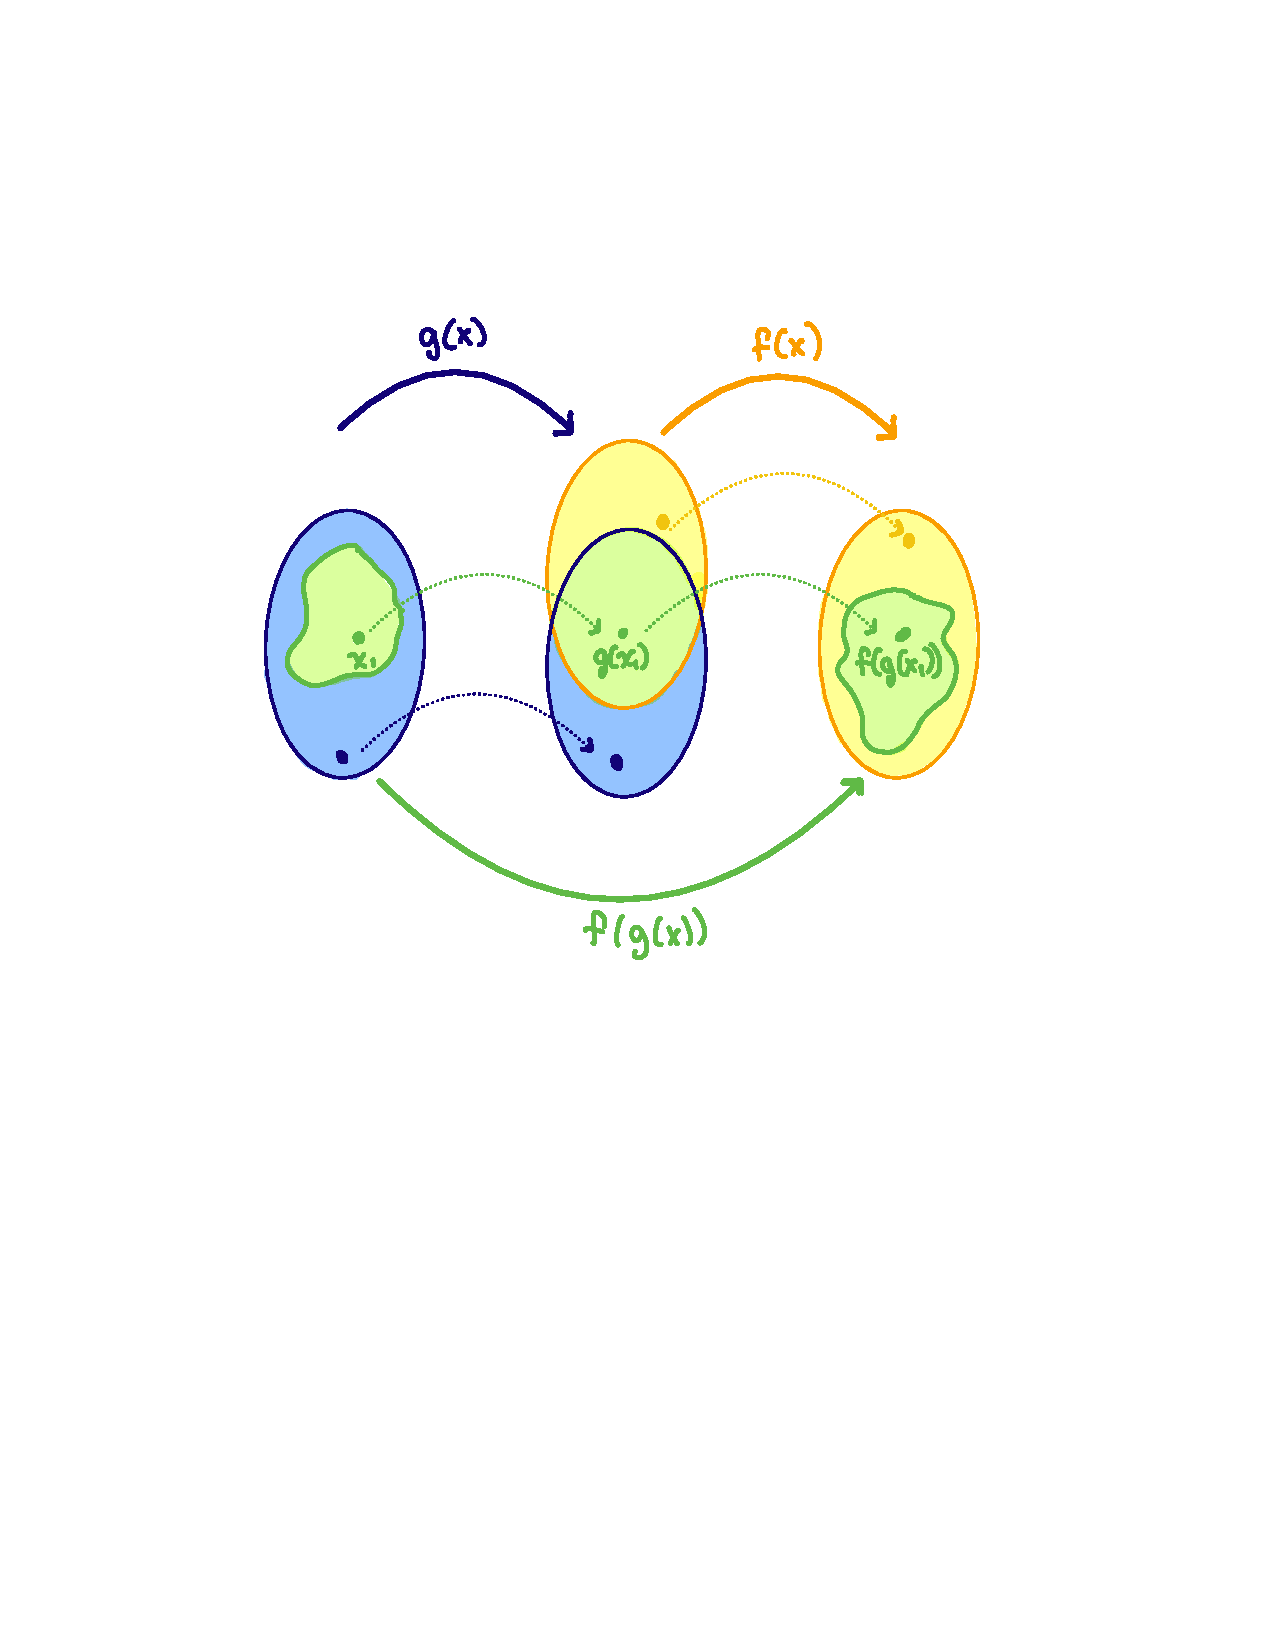
\includegraphics{CompDom1.pdf}
\end{image}



To find the domain of a composite function, $f\circ g$, you can follow these three steps:
\begin{enumerate}[label=\arabic*)]
\item Find the domain of $g$.
\item Find the domain of $f$.
\item Find those inputs $x$ in the domain of $g$ for which $g(x)$ is in the domain of $f$.  That is, exclude those inputs $x$ from the domain of $g$ for which $g(x)$ is not in the domain of $f$.  The resulting set is the domain of $f \circ g$.  
\end{enumerate} 

\begin{example}
Find the domain of $f \circ g$ where $f(x)=\frac{5}{x-1}$  and $g(x)=\frac{4}{3x-2}$.

\begin{explanation}
The domain of $g$ consists of all real numbers except $x=\frac{2}{3}$, since that input value would cause us to divide by 0. Likewise, the domain of $f$ consists of all real numbers except $1$. We need to exclude from the domain of $g$ any value of $x$ for which $g(x)=1$.


\begin{align*}
\frac{4}{3x-2} &=1\\
4 &=3x-2\\
6 &=3x\\
x &=2
\end{align*}

So the domain of $f \circ g$ is the set of all real numbers except $\frac{2}{3}$ and $2$. This means that

$$
x \neq \frac{2}{3} \text{ or } x \neq 2
$$

We can write this in interval notation as
$$
\left(-\infty,\frac{2}{3}\right) \cup \left(\frac{2}{3},2\right) \cup \left(2,\infty\right)
$$

\end{explanation}
\end{example}




\begin{example}
Find the domain of $f \circ g$ where $f(x)=\sqrt{x+2}$ and $g(x)=\sqrt{3-x}$.

\begin{explanation}

Because we cannot take the square root of a negative number, the domain of $g$ is $(-\infty,3]$. Now we check the domain of the composite function

$$
(f \circ g)(x)=\sqrt{\sqrt{3-x}+2}
$$

For $(f \circ g)(x)=\sqrt{\sqrt{3-x}+2}$, we need $\sqrt{3-x}+2 \geq 0$, since the inside of a square root cannot be negative. Since square roots are non-negative, $\sqrt{3-x} \geq 0$ sp $\sqrt{3-x}+2 \geq 0$ as long as $\sqrt{3-x}$ exists. That means $3-x \geq 0$, which gives a domain of $(- \infty,3]$.

\end{explanation}

\end{example}

This example shows that knowledge of the range of functions (specifically the inner function) can also be helpful in finding the domain of a composite function. It also shows that the domain of $f \circ g$ can contain values that are not in the domain of $f$, though they must be in the domain of $g$.

\begin{exploration}
Find the domain of $f \circ g$ where $f(x)=\frac{1}{x-2}$ and $g(x)=\sqrt{x+4}$.
\end{exploration}




%\typeout{************************************************}
%\typeout{Subsection Ranges of Composite Functions}
%\typeout{************************************************}

\section{Ranges of Composite Functions}
The range of a composite function such as $f \circ g$ is dependent on the range of $g$ and the range of $f$. It is important to know what values can result from a composite function, that is, to know the range of a function such as $f  \circ g$. 

Let us assume we know the ranges of the functions $f$ and $g$ separately. If we write the composite function for an input $x$ as $f(g(x))$, we can see right away that $f(g(x))$ must be a member of the range of $f$ since we will input the value $g(x)$ into $f$. However, we also see that it is possible that not all values in the range of $f$ are in the range of $f(g(x))$.  

\begin{image}
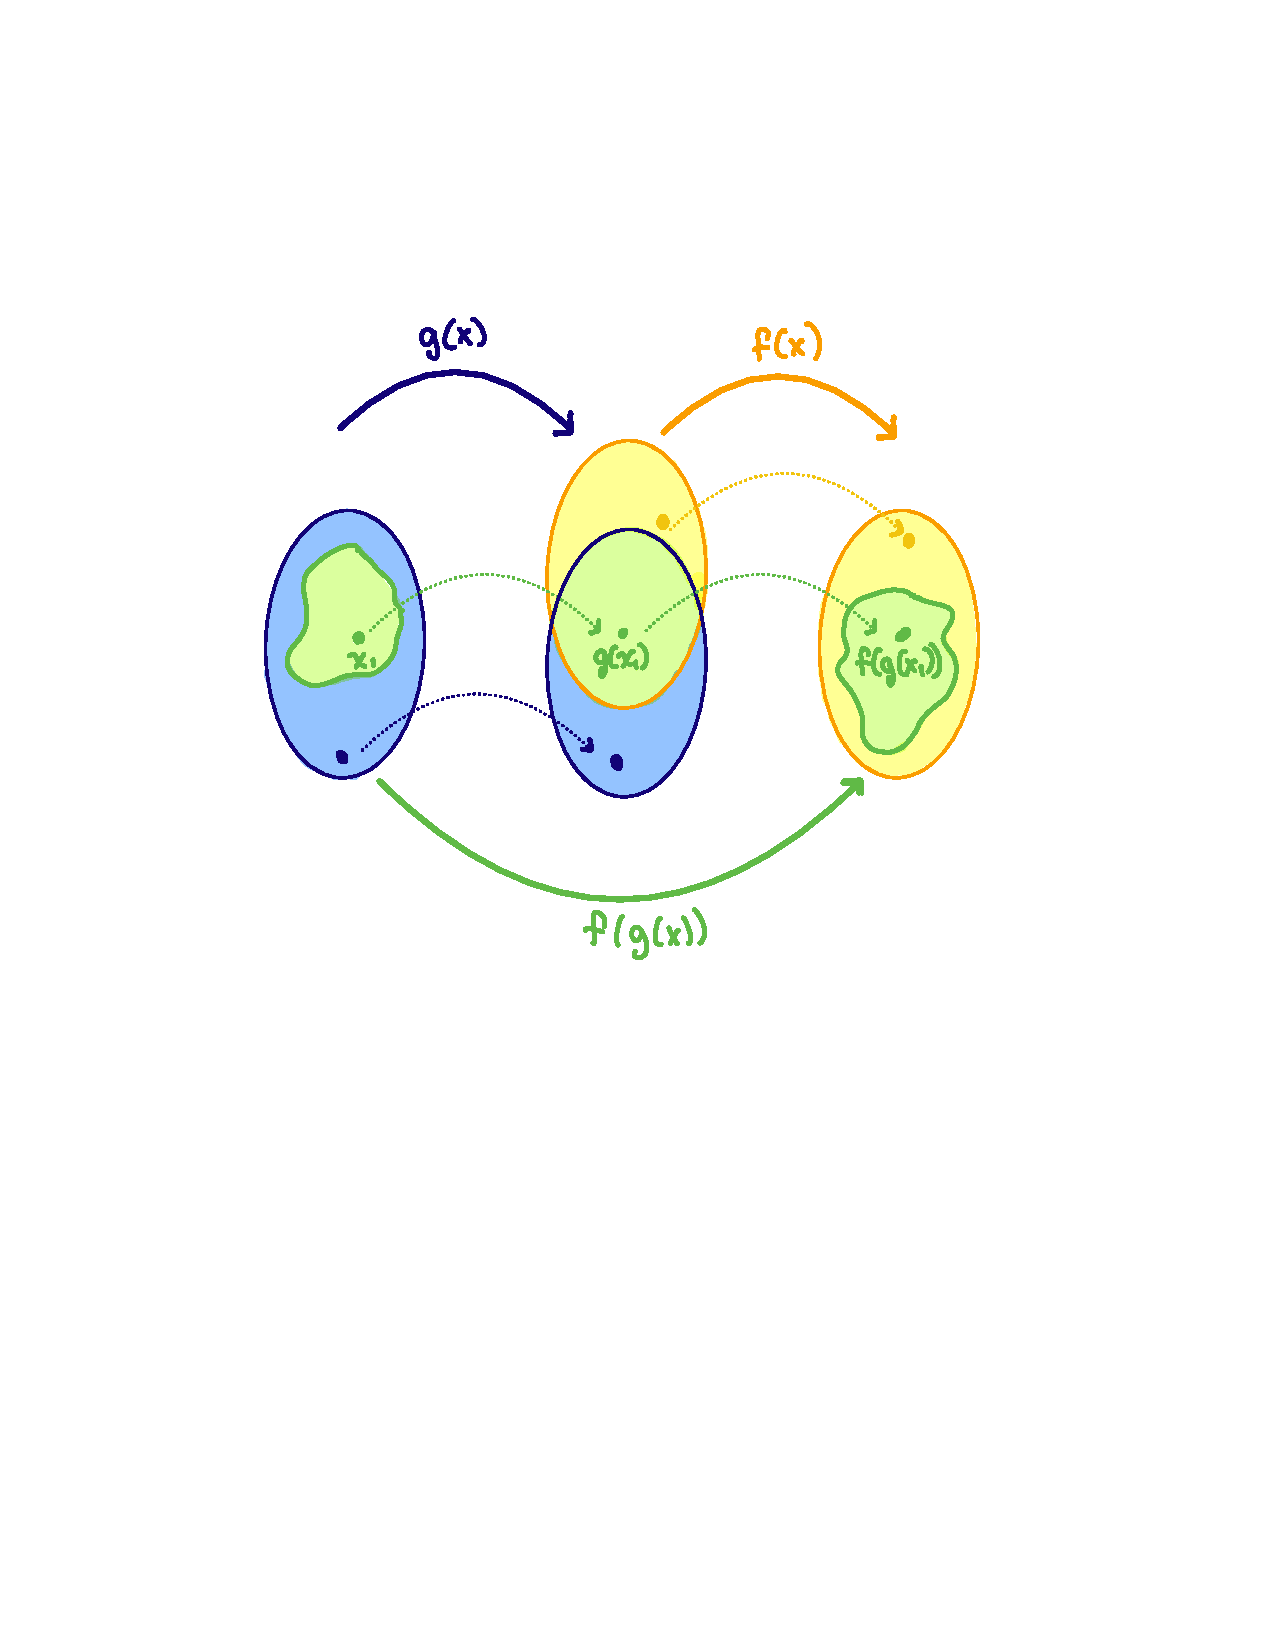
\includegraphics{CompDom1.pdf}
\end{image}

From the image above, we can see that there might be values in the yellow region which are in the range of $f$ but for which there are no $x$ values for which $f(g(x))$ gives that output.

\begin{callout}
	The range of a composite function $f\circ g$ is a subset of the range of $f$. 
\end{callout}

To find the domain of a composite function, $f \circ g$, you can follow these three steps:
\begin{enumerate}[label=\arabic*)]
	\item Find the range of $g$.
	\item Find the range of $f$.
	\item Restrict the domain of $f$ to the \emph{range} of $g$ and then determine the outputs of $f$ of these values.  
\end{enumerate} 


\begin{example}
Find the range of $f \circ g$ where $f(x)=\sqrt{x+2}$ and $g(x)=\sqrt{3-x}$.

\begin{explanation}
Because the output of a square root is always a positive number, the range of $g$ is $[0,\infty)$.  Similarly, the range of $f$ is $[0,\infty)$.  But now we must think about what happens when we restrict the input of $f$ to values in the range of $g$, $[0,\infty)$.  If $x \geq 0$, then $x+2 \geq 2$.  Taking the square root of both sides, we see that possible outputs of $f(g(x))$ will be $\sqrt{x+2} \geq \sqrt{2}$.  That is, the range of $f \circ g$ is $[\sqrt{2},\infty)$.

If we look at this function in Desmos, we can confirm graphically that this answer makes sense.  What we want to do is think about collapsing the graph unto the $y$-axis.  The range of the function will be the $y$-values that correspond to a point $(x,y)$ on the curve.  

First, we graph the function using a standard window.
\begin{image}
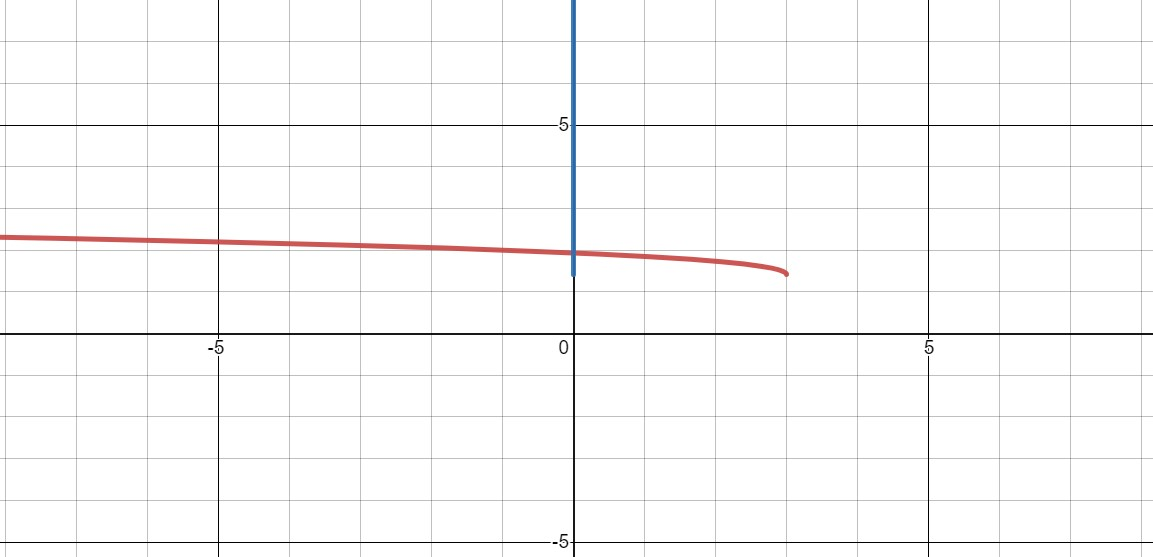
\includegraphics{composite-range.jpg}
\end{image}

This allows us to see the domain pretty well.  In the previous example, we found the domain to be $(- \infty,3]$ and if we collapse this function to the $x$-axis, it looks like the $x$-values that correspond to points on this curve are exactly the $x$ in $(- \infty,3]$.  If might be difficult to tell the domain from this graph, though.  Let's zoom out some.

\begin{image}
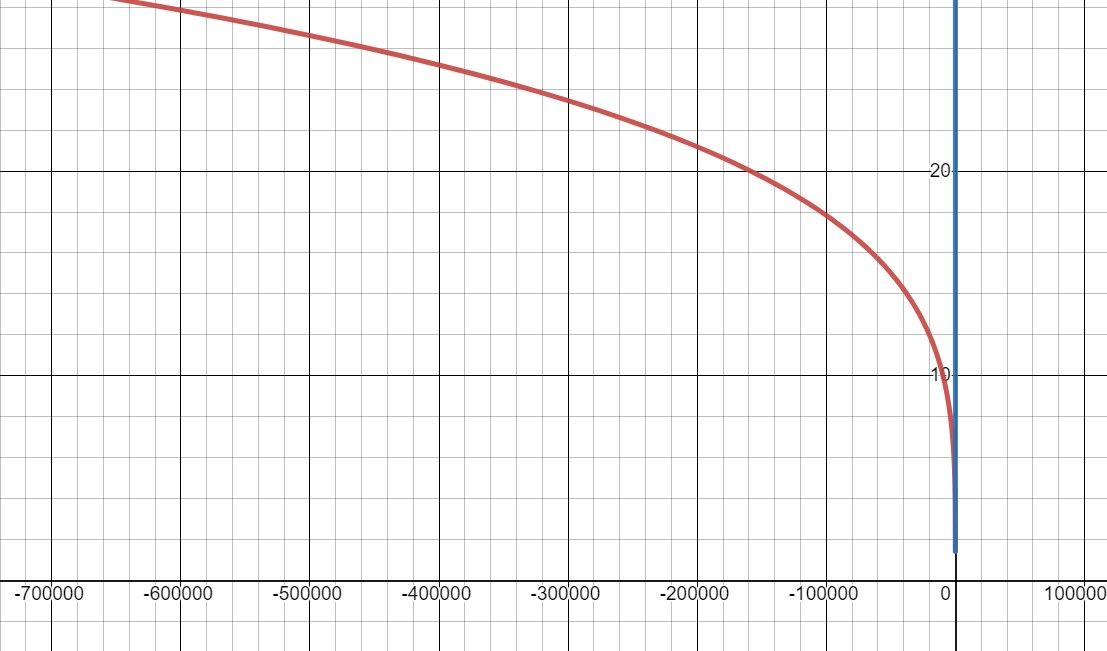
\includegraphics{composite-range-zoomed-out.jpg}
\end{image}

Here is the same graph in Desmos, so you can zoom in and out yourself.
\begin{center}  
\desmos{0wf1e4yyhf}{800}{600}  
\end{center}

You can now see that the blue line is showing this graph collapsed to the $y$-axis.  We can tell that the range will be positive numbers above some value between 1 and 2.  This corresponds with our result above of $[\sqrt{2},\infty)$.  In order to find the exact point $\sqrt{2}$ where the interval begins or to confirm that the interval really goes to infinity, we need to do the reasoning above.

\end{explanation}

\end{example}


\section{Composing $f(x)=x^2$ and $g(x)=\sqrt{x}$}

This final example is going to be a very important one that comes up often so we we will give it its own section.

\begin{example}
Let $f(x)=x^2$ and let $g(x)=\sqrt{x}$.  
\begin{enumerate}[label=\alph*.]
\item Find the domain and range of $f \circ g$ and compare this function to $id(x)=x$ and $abs(x)=|x|$.
\item Find the domain and range of $g \circ f$ and compare this function to $id(x)=x$ and $abs(x)=|x|$.
\end{enumerate}

\begin{explanation}
You probably have the idea that the squaring and squarerooting actions undo one another.  This is true for nonnegative values of $x$, but can get tricky when $x$ is allowed to be negative.  Let's look at each of these situations closely.
\begin{enumerate}[label=\alph*.]
\item First we consider $f \circ g$ and compare this function to $id(x)=x$ and $abs(x)=|x|$.  We have $f(x)=x^2$ and $g(x)=\sqrt{x}$ so 
$$(f \circ g)(x) = f(g(x))=(g(x))^2=(\sqrt{x})^2.$$ 

Let's consider the domain of this function.  Recall that the domain of a composite function $f \circ g$ is the set of those inputs $x$ in the domain of $g$ for which $g(x)$ is in the domain of $f$.  In this case, this means that the domain of $f(g(x))=(\sqrt{x})^2$ is the set of those inputs $x$ in the domain of $g(x)=\sqrt{x}$ for which $\sqrt{x}$ is in the domain of $f(x)=x^2$.  The implied domain of $g(x)=\sqrt{x}$ is $[0,\infty)$ since we cannot take the square root of a negative number.  Therefore, since the domain of the composition has to be only values in the domain of $g(x)$, this means the largest our domain can be is $[0,\infty)$.  Now, the only additional limiting factor is that the values $\sqrt{x}$ must be in the domain of $f$ but since the domain of $f$ is all real numbers, that will not limit the domain of the composition.  Therefore, the domain of $f \circ g$ is  $[0,\infty)$.

Now that we know the domain and we know that squaring and squarerooting undo each other for nonnegative values of $x$, we can conclude that $f \circ g$ is the identity function, $id(x)=x$ but restricted to the domain $[0,\infty)$.  That is,
$$(f \circ g)(x) =  (\sqrt{x})^2 = x, x \geq 0$$

Since the absolute value function is the same as the identity function when $x \geq 0$.  Therefore, we could also say that 
$$(f \circ g)(x) =  (\sqrt{x})^2 = |x|, x \geq 0$$

From this information, we also know that the range of $f \circ g$ will also be $[0,\infty)$, since $(f \circ g)(x) =  (\sqrt{x})^2$.

Here is a graph of $(f \circ g)(x) =  (\sqrt{x})^2$.

\begin{image}
  \begin{tikzpicture}
        \begin{axis}[
                    xmin=-5,xmax=7,
                    ymin=-5,ymax=7,
%                    xtick={2,4,...,14},
%                    minor xtick={1,2,...,15},
%                    ytick={100,200,300},
%                    minor ytick={20,40,...,320},
                    ]
            \addplot+[domain = 0:7,->]{x};
            \addplot[soliddot] coordinates {(0,0)} node[above left]{$(f \circ g)(x) =  (\sqrt{x})^2$};
        \end{axis}
\end{tikzpicture}
\end{image}

\item Now we consider $g \circ f$ and compare this function to $id(x)=x$ and $abs(x)=|x|$.  The domain of $g(f(x))=\sqrt{x^2}$ is the set of those inputs $x$ in the domain of $f(x)=x^2$ for which $x^2$ is in the domain of $g(x)=\sqrt{x}$.  The domain of $f(x)=x^2$ is all real numbers, so this does not reduce the domain of the composite function.  The range of $f(x)=x^2$ is $[0,\infty)$ since the square of every number will be greater than or equal to zero.  The implied domain of $g(x)=\sqrt{x}$ is $[0,\infty)$.  Therefore, every output from $f(x)=x^2$ is in the domain of $f(x)=\sqrt{x}$.  Therefore, the domain of $g \circ f$ is  $(-\infty,\infty)$.

Now, let's consider the range of $g \circ f$.  We know that the range of $g \circ f$ must be contained in the range of $g(x)=\sqrt{x}$.  The range of $g(x)=\sqrt{x}$ is $[0,\infty)$, so that is the largest range possible for $g \circ f$.  We know that for values of $x \geq 0$, squaring and squarerooting undo one another so we know that all the values of $[0,\infty)$ are contained in the range of $g \circ f$.  More precisely, for any value $x_0$ in $[0,\infty)$, $g(f(x_0))=x_0$ so $x_0$ will be in the range of $g \circ f$.  Thus, the range of $g \circ f$ is $[0,\infty)$.

Now, since we know that this function $g \circ f$ only outputs positive numbers, we know it cannot equal the identity function for inputs of $x<0$.  Let's explore what this function does for values of $x<0$ by considering $x=-2$.

$$g(f(-2))=\sqrt{(-2)^2}=\sqrt{4}=2$$

Notice, that we input $x=-2$ but the output was positive 2.  In fact, for all values of $x<0$, $g(f(x))=\sqrt{x^2}=-x=|x|$.

Since the absolute value function is the same as the identity function when $x \geq 0$ but the negative of the idenity function for $x<0$, we have that 
$$(g \circ f)(x) =  \sqrt{x^2} = |x|$$

Here is a graph of $(g \circ f)(x) =  \sqrt{x^2} = |x|$.

\begin{image}
  \begin{tikzpicture}
        \begin{axis}[
                    xmin=-7,xmax=7,
                    ymin=-7,ymax=7,
%                    xtick={2,4,...,14},
%                    minor xtick={1,2,...,15},
%                    ytick={100,200,300},
%                    minor ytick={20,40,...,320},
                    ]
            \addplot+[domain = 0:7,->, color=penColor]{x};
            \addplot+[domain = -7:0,<-, color=penColor]{-x};
            \addplot[soliddot, color=penColor] coordinates {(0,0)};
        \end{axis}
\end{tikzpicture}
\end{image}
\end{enumerate}
\end{explanation}

\end{example}

%\typeout{************************************************}
%\typeout{Summary}
%\typeout{************************************************}

\begin{summary}\begin{itemize}
\item For a composite function $f \circ g$ to be defined, we need outputs of $g$ to be among the allowed inputs for $f$.  In particular, if the range of $g$ is a subset of the domain of $f$, we can say that if $g : A \to B$ and $f : B \to C$, then $f \circ g : A \to C$.  In this case, the domain of the composite function is the domain of the inner function, and the range of the composite function is the codomain of the outer function.
\item In general, the domain of a composite function $f \circ g$ is the set of those inputs $x$ in the domain of $g$ for which $g(x)$ is in the domain of $f$. 
\item In general, the range of a composite function $f \circ g$ is a subset of the range of $f$. 
\end{itemize}\end{summary}




\end{document}
